\chapter[Simulado 4]{Simulado}

\num{1} Um jogo consiste em uma pessoa sortear um número e, depois de ver
que número é esse, pensar por alguns instantes e dizer em qual potinho
deve ser colocado cada algarismo do número.

\begin{figure}[htpb!]
\centering
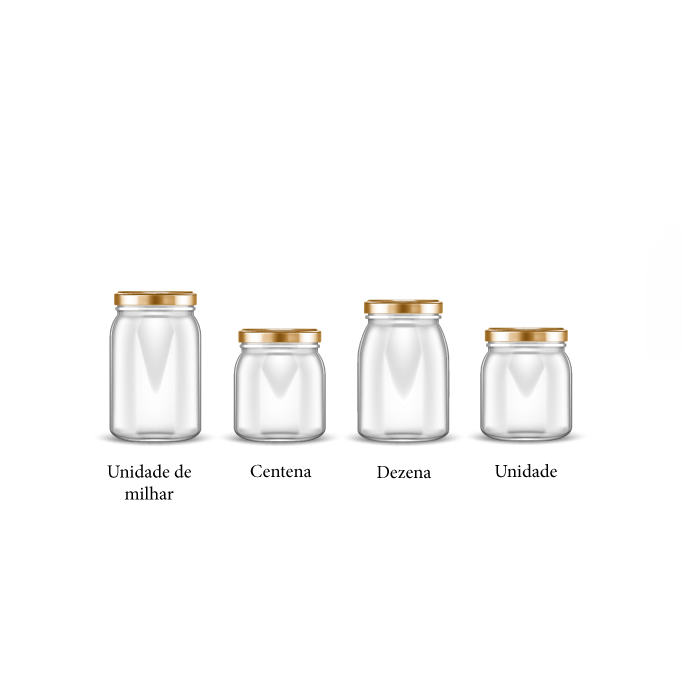
\includegraphics[width=.8\textwidth]{../ilustracoes/MAT5/SAEB_5ANO_MAT_figura123.png}
\end{figure}

O número que acabou de ser sorteado foi 3.756. Que algarismo será
colocado no potinho com rótulo centenas?

%\begin{minipage}{.5\textwidth}
\begin{escolha}
\item
  7
\item
  6
\item
  5
\item
  3
\end{escolha}
%\end{minipage}



\num{2} Jorge foi passar férias no sítio pertencente a sua família.
Chegando lá, correu até a horta e colheu 10 dezenas de pés de rúcula, 1
centena de espigas de milho, 5 dezenas de tomate, 2 unidades de cebola e
3 pepinos. Qual o total de produtos colhidos por Jorge?

%\begin{minipage}{.5\textwidth}
\begin{escolha}
\item
  21
\item
  255
\item
  405
\item
  675
\end{escolha}
%\end{minipage}



\num{3} Geraldo queria enviar um presente ao amigo José que mudou de
cidade. Ele se lembrava do nome da rua para a qual o amigo havia se 
mudado, mas não sabia qual o número da casa. Geraldo então enviou
uma mensagem ao amigo perguntando o número da casa e José respondeu da
seguinte maneira:

\begin{figure}[htpb!]
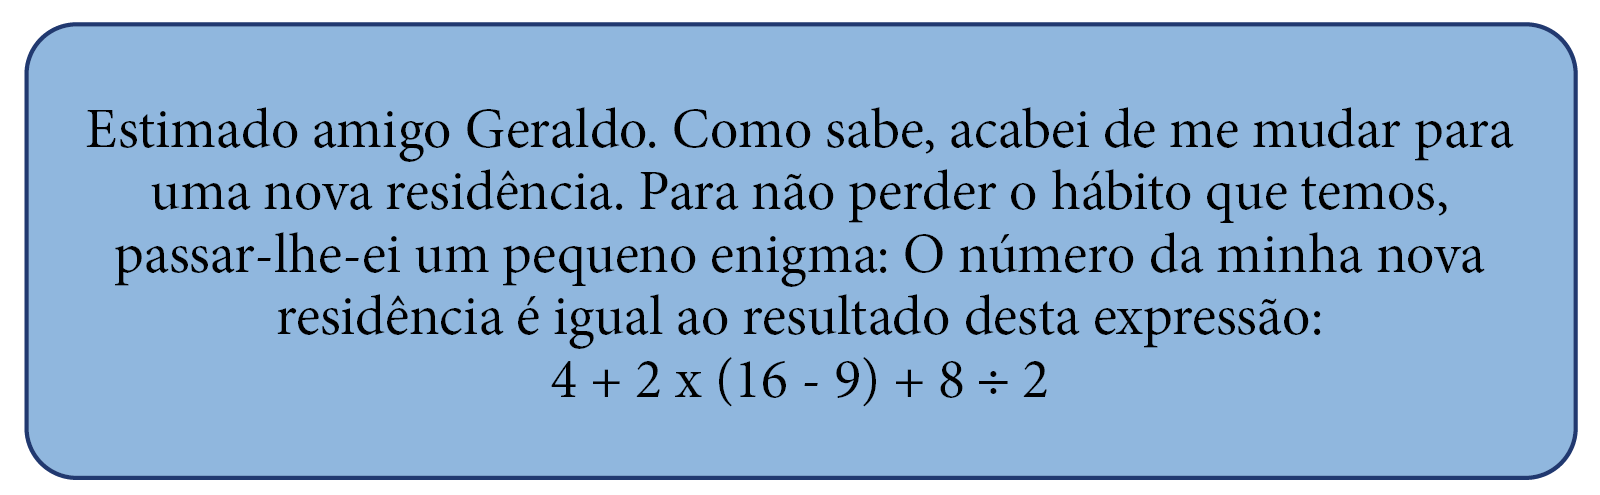
\includegraphics[width=\textwidth]{../ilustracoes/MAT5/SAEB_5ANO_MAT_figura124.png}
\end{figure}

%Acredito que haja um problema com este gabarito. A montagem da expressão numérica, sem distinção de parênteses e colchetes, permite chegar a mais de um resultado. Prefiro deixar essa avaliação para os leitores críticos. Provavelmente eles farão vários reparos, inclusive em páginas anteriores. (Rogério, 5/4/23, 9h07)

Qual o número da casa de José?

\begin{multicols}{4}
\begin{escolha}
\item
  13
\item
  20
\item
  22
\item
  28
\end{escolha}
\end{multicols}


\enlargethispage{2\baselineskip}
\num{4} Arnaldo esqueceu um dos números que fazem parte da senha do cofre
que tem em casa. Ele lembra que a senha era composta por 6
números e que os números da senha formam a seguinte sequência (2, 102,
202, \_\_A\_\_, 402, 502).

Através da análise da sequência podemos afirmar que o número A, o qual
ele esqueceu é:

\begin{multicols}{2}
\begin{escolha}
\item
  O dobro de 150
\item
  O antecessor de 303
\item
  O sucessor de 251
\item
  Metade de 500
\end{escolha}
\end{multicols}



\num{5} Considerando que todos os objetos abaixo estão cheios de água,
qual deles pode conter exatamente 3 litros de água?

\begin{figure}[htpb!]
\centering
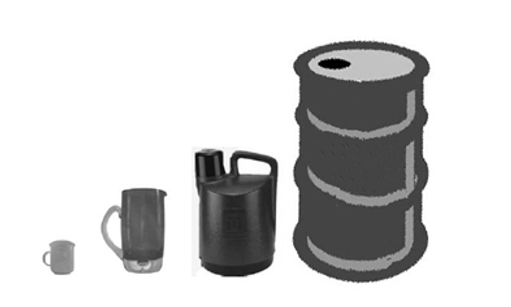
\includegraphics[width=.5\textwidth]{./imgs/mat22.png}
\end{figure}

%Pessoalmente julgo esta questão bastante ruim, baseada apenas no senso-comum, sem qualquer fundamento além dele. Tudo é discutível nesta questão, tudo depende da subjetividade. (Rogério, 5/4/23, 9h13)

\begin{multicols}{4}
\begin{escolha}
\item
  A caneca
\item
  A jarra
\item
  O garrafão
\item
  O tambor
\end{escolha}
\end{multicols}


\pagebreak
\num{6} Observe as figuras representadas na malha quadriculada abaixo:

\begin{figure}[htpb!]
\centering
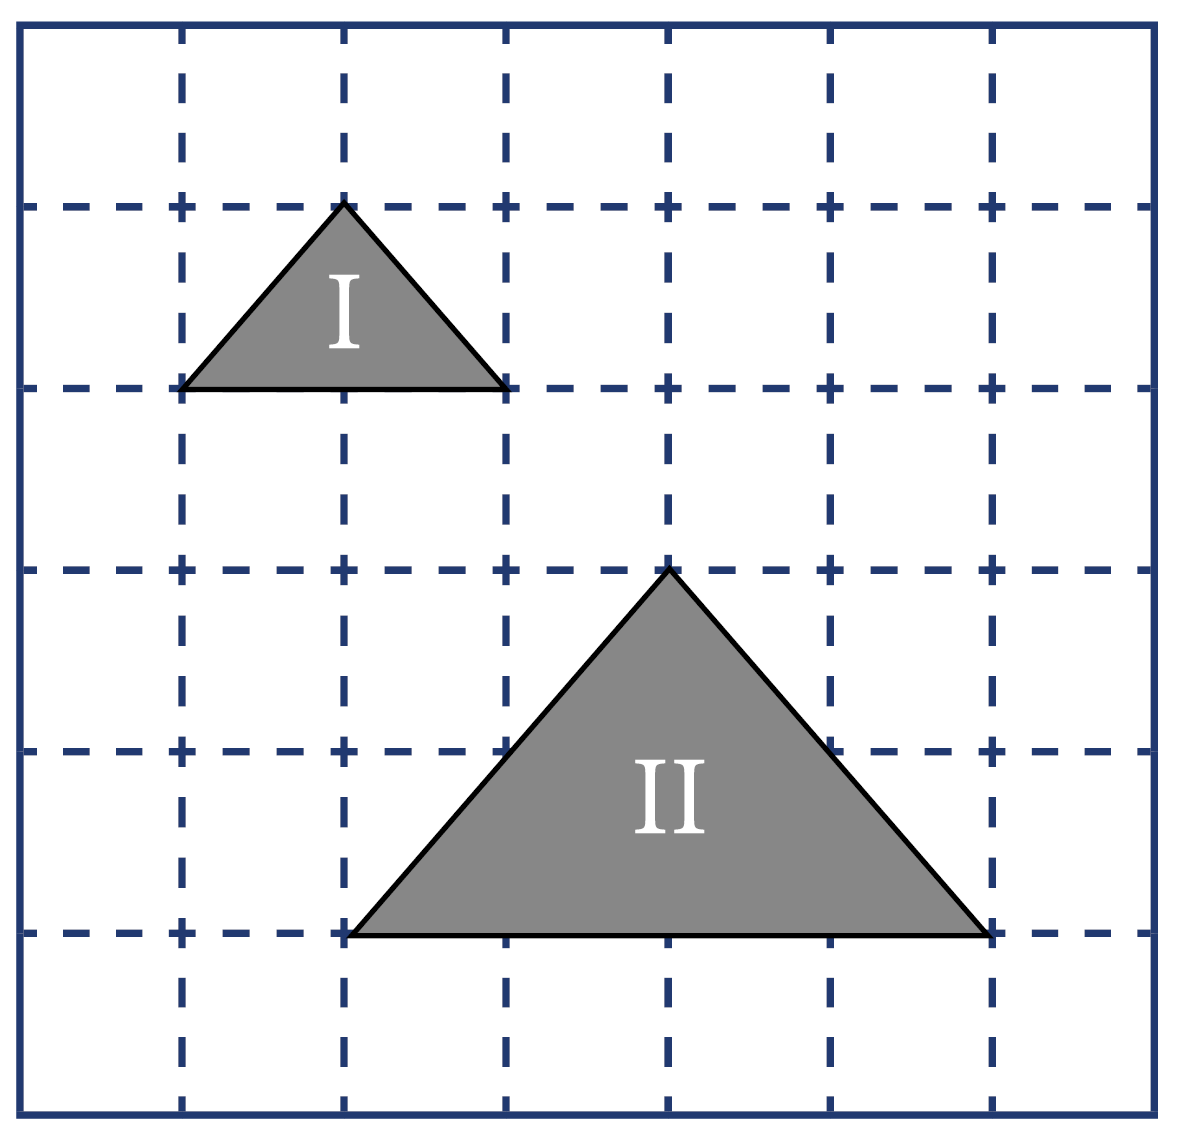
\includegraphics[width=.7\textwidth]{../ilustracoes/MAT5/SAEB_5ANO_MAT_figura125.png}
\end{figure}

Sabe-se que a figura II é um ampliação da figura I. O perímetro da
figura II, em relação ao perímetro da figura I, ficou:

%\begin{minipage}{.5\textwidth}
\begin{escolha}
\item
  Reduzido à metade
\item
  Inalterado
\item
  Duplicado
\item
  Quadruplicado
\end{escolha}
%\end{minipage}


\num{7} Rafael foi a uma papelaria e comprou um livro por R\$ 35,00 e uma
caneta por R\$ 3,00. Das alternativas abaixo, qual pode representar as
cédulas e moedas que Rafael utilizou para pagar, sabendo-se que não terá
troco?

\begin{escolha}
\item
  1 cédula de 10 reais, 5 cédulas de 5 reais e 3 moedas de 1 real.
\item
  1 cédula de 10 reais, 4 cédulas de 5 reais e 3 moedas de 1 real.
\item
  2 cédulas de 10 reais, 1 cédulas de 5 reais e 3 moedas de 1 real.
\item
  2 cédulas de 10 reais, 2 cédulas de 5 reais e 2 moedas de 1 real.
\end{escolha}



\pagebreak
\num{8} Alana resolveu trocar todas as moedas que estavam em seu cofrinho
por uma única cédula. Ela tinha no cofrinho 10 moedas de 5 centavos, 5
moedas de 50 centavos, 70 moedas de 10 centavos.

Marque a alternativa que trás a nota correta que substituiu em valor
todas as moedas que Alana tinha em seu cofrinho:

\begin{figure}[htpb!]
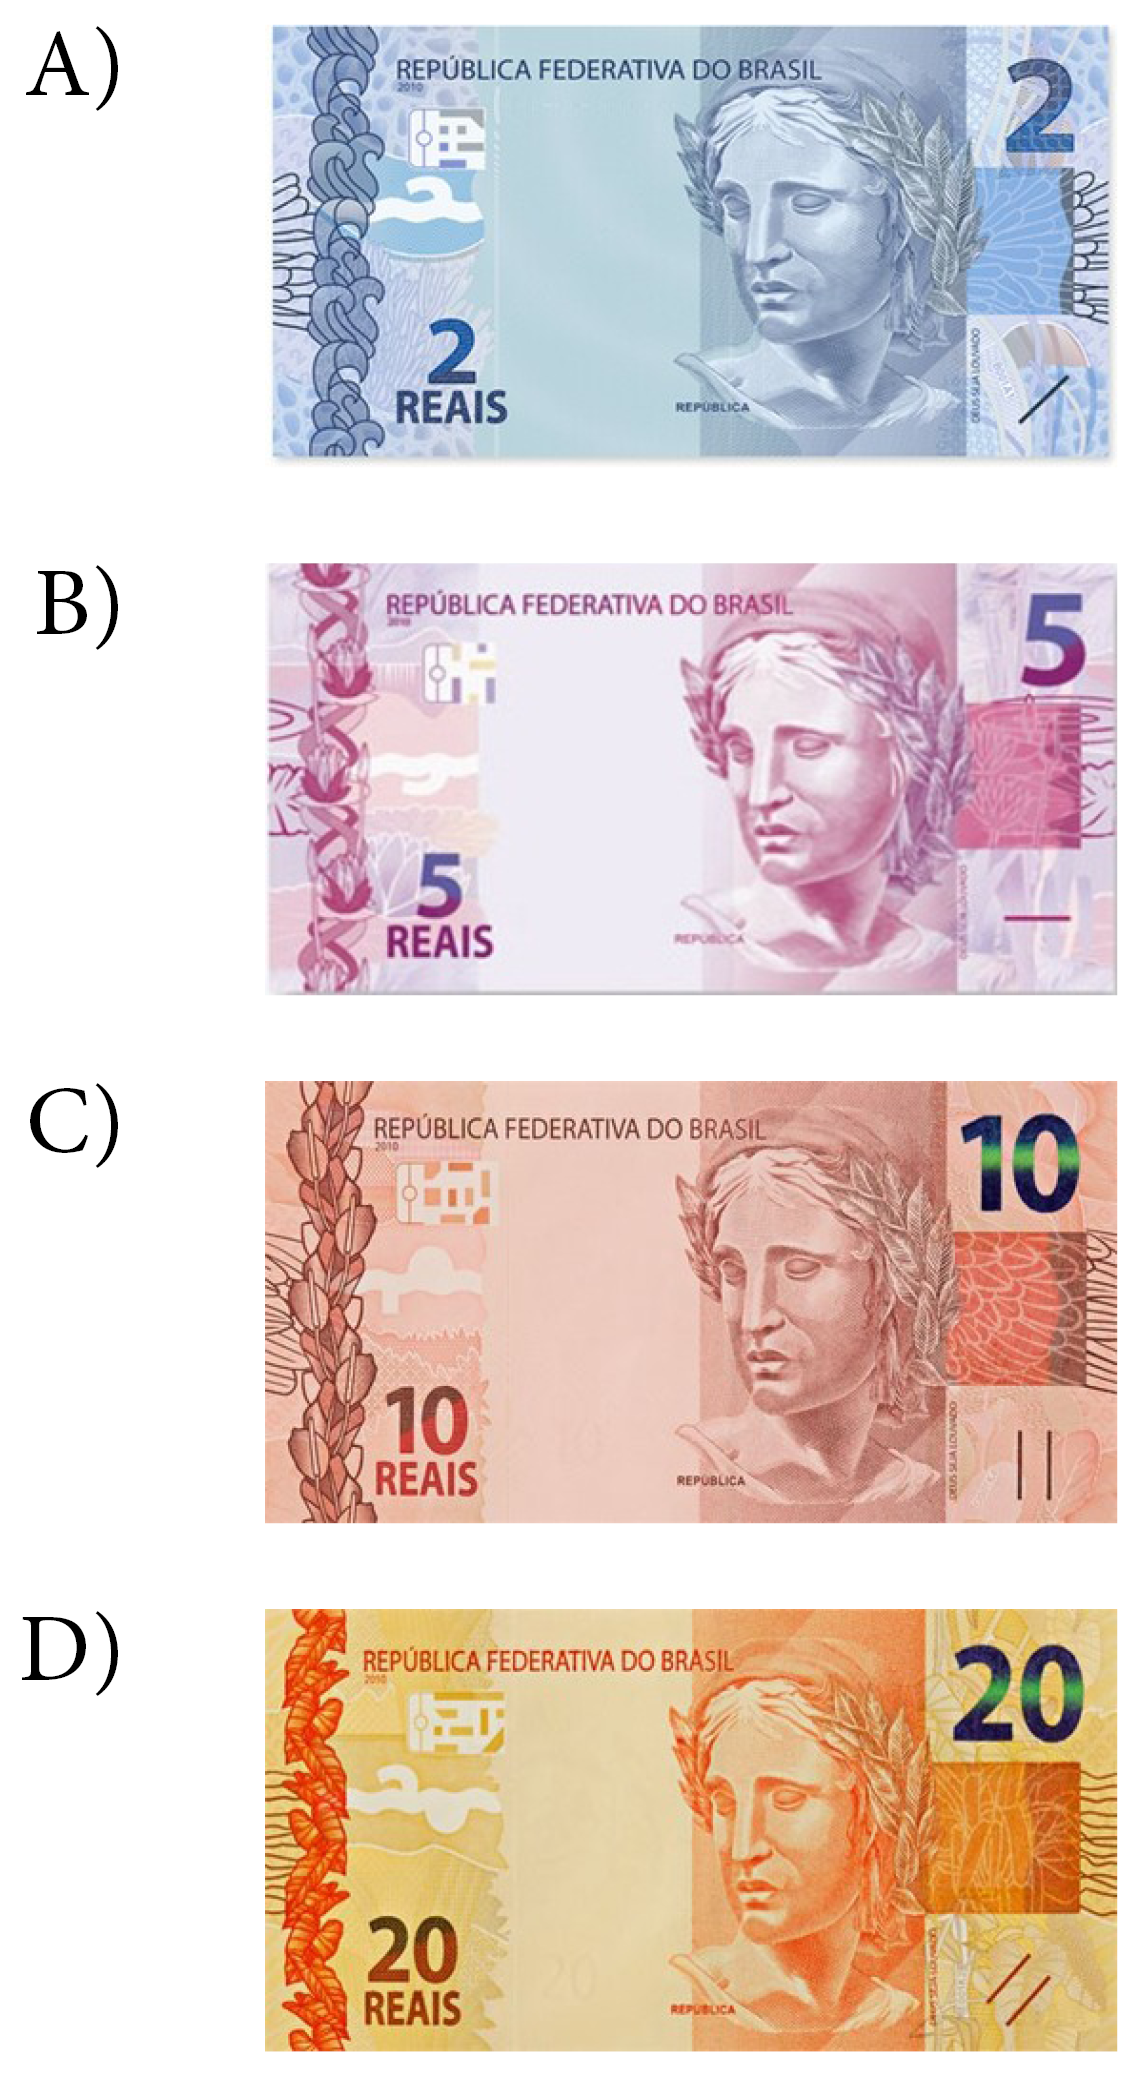
\includegraphics[width=.4\textwidth]{../ilustracoes/MAT5/SAEB_5ANO_MAT_figura126.png}
\end{figure}



\num{9} Dentre os números naturais distintos de 1 a 20, escolhe-se um ao
acaso. Qual a probabilidade de se escolher um número par?

\begin{escolha}
\item
  10\%
\item
  35\%
\item
  50\%
\item
  90\%
\end{escolha}


\num{10} Em uma compeção de saltos ornamentais, cada atleta tem direito
a 3 saltos e sua pontuação final é dada pela soma dos 3 saltos. Ganha a
prova quem fizer o maior número de pontos no total.

A tabela abaixo mostra as notas obtidas por 5 atletas, A, B, C, D e E,
nos seus respectivos saltos:

\begin{center}
\begin{tabular}{l|c|c|c}
\hline
\textbf{Atleta} & \multicolumn{1}{l|}{\textbf{Pontuação do 1º salto}} & \multicolumn{1}{l|}{\textbf{Pontuação do 2º salto}} & \multicolumn{1}{l}{\textbf{Pontuação do 3º salto}} \\ \hline
\textbf{A} & 6 & 6 & 6 \\ \hline
\textbf{B} & 7 & 3 & 8 \\ \hline
\textbf{C} & 5 & 7 & 6 \\ \hline
\textbf{D} & 5 & 6 & 8 \\ \hline
\end{tabular}
\end{center}

Analisando as notas de cada um dos atletas, podemos dizer que o campeão
foi o atleta:

\begin{escolha}
\item
  A
\item
  B
\item
  C
\item
  D
\end{escolha}


\num{11} Em uma prova de automobilismo, o piloto que estava em
primeiro lugar sofreu com falta de combustível e precisou abandonar a
prova quando já tinha completado 2/7 da prova de 77 voltas no total.
Pode-se dizer que ele abandonou a prova depois de ter percorrido:

%\begin{minipage}{.5\textwidth}
\begin{escolha}
\item
  11 voltas
\item
  22 voltas
\item
  30 voltas
\item
  44 voltas
\end{escolha}
%\end{minipage}


\num{12} Em uma mapa, a distância de 2.000 km entre duas cidades foi
representada por 16 cm. Qual a razão entre o valor desenhado no
mapa e a distância real entre as cidades?

%\begin{minipage}{.5\textwidth}
\begin{escolha}
\item
  125
\item
  1/250
\item
  1/125
\item
  250
\end{escolha}
%\end{minipage}


\pagebreak
\num{13} Quantos números formados por 2 algarismos podemos formar com os
algarismos 1; 2; 3; 4; 5; 6; 7; 8 e 9 de forma que nenhum algarismo seja
repetido?

\begin{multicols}{2}
\begin{escolha}
\item
  81
\item
  72
\item
  100
\item
  64
\end{escolha}
\end{multicols}


\num{14} Alexandre foi até uma loja comprar um tênis e foi informado de 
que o valor era de R\$ 324,80. Após algum tempo de negociação, a loja
resolveu abaixar o preço em R\$ 32,40 e parcelar o restante em 4 vezes de
mesmo valor cada parcela. Alexandre aceitou a negociação.

Qual o valor de cada parcela que Alexandre irá pagar?

%\begin{minipage}{.5\textwidth}
\begin{escolha}
\item
  R\$ 112,60
\item
  R\$ 96,54
\item
  R\$ 73,10
\item
  R\$ 32,40
\end{escolha}
%\end{minipage}


\num{15} Leia o texto.
\begin{myquote}
  {[}\ldots{}{]} Semba: é uma dança de salão angolana urbana. Dançada em pares, com
  passadas distintas dos cavalheiros, seguidas pelas damas em passos
  totalmente largos, onde o malabarismo dos cavalheiros conta muito para
  o nível de improvisação. O Semba caracteriza-se como uma dança de
  passadas. Não é ritual nem guerreira, mas de divertimento,
  principalmente em festas. {[}\ldots{}{]}

\fonte{Secretaria da Educação do Estado do Paraná. Danças Africanas. Disponível
em: \emph{
http://www.educacaofisica.seed.pr.gov.br/modules/conteudo/conteudo.php?conteudo=62}.
Acesso em: 16 fev. 2023.}
\end{myquote}

\noindent{}Depois de ler o texto, nota-se que se trata de uma prática corporal que tem semelhança
com o samba. O motivo é que as duas danças são

\begin{escolha}
\item realizadas no carnaval.

\item originárias da cultura africana.

\item atividades competitivas.

\item praticadas em eventos religiosos
\end{escolha}



\pagebreak
\num{16} A seguir, aparece um trecho de notícia. Leia-a.
\begin{myquote}
  O Governo do Paraná vai levar as artes marciais para dentro das
  escolas estaduais, oferecendo treinamentos no contraturno às aulas
  convencionais {[}\ldots{}{]}

A ideia, explicou o governador, é começar o projeto-piloto no segundo semestre {[}\ldots{}{]} “Gosto muito do esporte, sou
um praticante. As artes marciais ensinam a filosofia do respeito, a
obedecer a hierarquia, a ser uma pessoa do bem” {[}\ldots{}{]}

Além da introdução de artes marciais nas escolas estaduais, há outra
iniciativa que diz respeito ao Japs Combat, espécie de Jogos Abertos do
Paraná, voltado apenas para as artes marciais. {[}\ldots{}{]}

\fonte{Paraná vai levar as artes marciais para dentro das escolas. Agência
Estadual de Notícias. Disponível em: \emph{
https://shorturl.at/egoHS}.
Acesso em: 16 fev. 2023.}
\end{myquote}

\noindent{}Depois de ler a notícia, nota-se que o objetivo das artes marciais é

\begin{escolha}
\item ensinar valores éticos aos alunos.

\item incentivar competições.

\item formar novos atletas.

\item aumentar os conflitos entre os alunos.
\end{escolha}



\num{17}
\begin{myquote}
  {[}\ldots{}{]} Por volta de 1880, jogadores de um clube inglês improvisaram
  um novo jogo por causa do mau tempo. Sobre uma mesa de sinuca, com
  livros como raquetes, um barbante como rede e uma bola de tênis
  normal, surgiram as primeiras raquetadas do tênis de mesa. {[}\ldots{}{]}


\fonte{Prefeitura de Lençóis Paulista. Tênis de mesa. Disp. em: \emph{
https://shorturl.at/jpE29}.
Acesso em: 16 fev. 2023.}
\end{myquote}

\noindent{}Com base no texto, percebe-se que o tênis de mesa, antes de ser um esporte olímpico, era

\begin{escolha}
\item uma atividade adaptada do tênis de campo.

\item uma modalidade esportiva.

\item um treinamento para usar as raquetes.

\item uma prática corporal para competição.
\end{escolha}



\pagebreak
\num{18} Em dias quentes de verão, observam-se altas temperaturas
nas manhãs e tardes, e fortes chuvas nas noites e nos dias seguintes. A
explicação desse fenômeno reside no fato da umidade do ar se elevar
nessa época do ano em comparação com outras estações.

O ar se torna mais úmido nesse período pois

\begin{escolha}
\item a evaporação e a evapotranspiração acontecem com maior intensidade.

\item a intensidade da luz solar impede chuvas mais frequentes.

\item o acúmulo de vapor de água nas nuvens é incomum em dias quentes.

\item o sol participa da formação de gotículas de água antes da chuva.
\end{escolha}



\num{19} Pequenos agricultores decidiram substituir as bombas d'água
que utilizavam água tratada para a irrigação das plantações. No lugar de
utilizar a água que vinha das companhias fornecedoras, criaram um tanque
para depositar água residual proveniente de atividades diárias que
desperdiçam água, goteiras e outras atividades agrícolas, como a própria
irrigação. Algumas espécies vegetais capazes de filtrar as impurezas da
água também foram utilizadas num pequeno circuito de tratamento.

A reutilização da água, nessas condições, é possível pois

\begin{escolha}
\item as plantações podem sobreviver com qualquer tipo de água.

\item o pequeno agricultor não trabalha com grandes plantações.

\item a irrigação representa o uso da água para um fim não potável.

\item a água de reúso é mais importante para o crescimento de vegetais.
\end{escolha}

\num{20} A digestão dos alimentos começa na boca, e o sistema
digestório é capaz de selecionar os nutrientes necessários para o
funcionamento do organismo e a produção de energia, dividindo os
alimentos em partículas menores. O oxigênio, inalado na inspiração,
participa da produção de energia no aproveitamento dos nutrientes,
enquanto o coração bombeia o sangue concentrado nos nutrientes divididos
para todos os tecidos do organismo humano.

A ação dos sistemas digestório, respiratório e circulatório após a
alimentação demonstra que

\begin{escolha}
\item o sistema respiratório é menos importante no processo de nutrição.

\item os sistemas atuam em conjunto no organismo humano.

\item a produção de energia poderia ser realizada somente pelo estômago.

\item o organismo pode sobreviver sem alimentos por muito tempo
\end{escolha}


\blankpage